\subsection{Trick to compute line integrals easily}
\begin{itemize}
    \item Apply Cauchy theorem \textrightarrow find simply connex set $u$ 'enclosing' loop $\gamma$ on which $f$ is holomorphic
    \item Apply extension of the Cauchy theorem \textrightarrow replace $\int_{\gamma_0}fdz$ over a 'very complicated' $\Gamma_0$ by $\int_{\gamma_1}fdz$ over a 'simpler' $\Gamma_1$
    \item If $\Gamma_0, \Gamma_1$ have some endpoint and orientation and $f$ is holomorphic on the region they enclose. Then:
		\begin{align*} \int_{\Gamma_0}fdz =  \int_{\Gamma_1}fdz \end{align*}
\end{itemize}

\begin{parag}{Extension of Cauchy's integral formula}
    Under the same hypothesis as for the Cauchy's integral formula:
	\begin{theoreme}
	\begin{align*} 
		f^{\left(n\right)}\left(z_0\right) =  \frac{n!}{2\pi i}\int_{\gamma}\frac{f\left(z\right)}{\left(z - z_0\right)^{\left(n + 1\right)}}dz
	\end{align*}
	\end{theoreme}
	\begin{subparag}{Remark}
	    And we can see that if $n = 0$ then this fall under the usual formula.
	\end{subparag}
	This gives us another way to compute a maybe 'complicated' using something that 'may' be easier.\\
	$ $\\
	This essentially follows by differentiating the Cauchy's integral formula
	\begin{proof}
		We first start from the Cauchy integral Formula:
		\begin{align*} 
			f\left(z_0\right) = \frac{1}{2\pi i}\int_{\gamma}\frac{f\left(z\right)}{z - z_0}dz
		\end{align*}
		We can take the derivative on both side
		\begin{align*} 
			f'\left(z\right) = \frac{1}{2\pi i}\frac{d}{d z_0} \int_{\gamma} \frac{f\left(z\right)}{z - z_0}dz
		\end{align*}
		Using Leibniz rule, we move the derivative inside the integral:
		\begin{align*} 
			f'\left(z_0\right) = \frac{1}{2 \pi i} \int_{\gamma} \frac{\partial }{\partial z_0} \left(\frac{f\left(z\right)}{z - z_0}\right)dz
		\end{align*}
		Since $f\left(z\right)$ does not depend on $z_0$, only the denominator is differentiated, which means that we need to compute:
		\begin{align*} 
			\frac{df}{dz_0} \left(z - z_0\right)^{-1} = \left(z - z_0\right)^{-2}
		\end{align*}
		Now if we substitutes this into our equation
		\begin{align*} 
			f'\left(z_0\right) =  \frac{1}{2\pi i} \int_{\gamma} \frac{f\left(z\right)}{\left(z - z_0\right)^2}
		\end{align*}
		Now to prove the general result (not only the base case) we will need to do the induction steps. Assume that $f^{\left(n\right)}\left(z_0\right) =  \frac{n!}{2\pi i}\int_{\gamma}\frac{f\left(z\right)}{\left(z - z_0\right)^{n + 1}}dz$. If we retake its derivative as before we have 
		\begin{align*} 
			f^{\left(n + 1\right)}\left(z_0\right) &= \frac{n!}{2\pi i} \frac{d}{dz_0} \int_{\gamma} \frac{f\left(z\right)}{\left(z - z_0\right)^{n + 1}}dz\\
												   &= \frac{n!}{2\pi i}\int_{\gamma} \frac{\partial }{\partial z_0} \frac{f\left(z\right)}{\left(z - z_0\right)^{n+1}}
		\end{align*}
		Let us now compute:
		\begin{align*} 
			\frac{\partial }{\partial z_0} \frac{1}{\left(z - z_0\right)^{n+1}} = - - \frac{n + 1}{\left(z - z_0\right)^{n + 2}}
		\end{align*}
		which gives us:
		\begin{align*} 
			f^{\left(n+1\right)}\left(z_0\right) = \frac{\left(n + 1\right)!}{2\pi i} \int_{\gamma} \frac{f\left(z\right)}{\left(z - z_0\right)^{\left(n + 1\right) + 1}}dz
		\end{align*}
	\end{proof}
\end{parag}
\begin{framedremark}
	This formula is used to prove a statement that we have already seen: holomorphic functions are infinitely many times differentiable.
\end{framedremark}
\begin{parag}{Example}
    Let $f\left(z\right) = \frac{\cos\left(z\right)}{z}$ and let $\gamma$ be a simple closed curve, oriented counter-clockwise. The question that we are trying to answer is: what are the value of $\int_{\gamma}fdz$?\\
	$ $\\
	Before starting anything we can see our function kind look like what is being integrated above. Knowing that we can first check some information about our function:
	\begin{itemize}
	    \item If $0 \in \gamma$ this integral is ill-defined
	    \item If $0 \notin \gamma$ and $0$ is not in the interior of $\gamma$ then we have that our function is holomorphic even inside the curve. Therefore by Cauchy integral theorem:
			\begin{align*} 
				\int_{\Gamma} fdz = 0
			\end{align*}
			\item If $0 \notin \gamma$ yet $0$ is in the interior of $\gamma$ then we note
				\begin{align*} 
					\int_{\gamma} f\left(z\right)dz &= \int_{\gamma}\frac{g\left(z\right)}{z} dz
				\end{align*}
				By the Cauchy integral formula for $g\left(z\right) =  \cos\left(z\right)$ and $z_0 = 0$ this gives us 
				\begin{align*} = 2\pi i g\left(0\right) =  2\pi i \end{align*}
	\end{itemize}
\end{parag}
\begin{parag}{Example II}
    Let $\gamma$ be the circle $\left\{z \in \mathbb{C}: \left\|z - 2\right\|= 1\right\}$ oriented counter-clockwise. Compute $\int_{\gamma}\frac{e^{z}}{\left(z - 2\right)^{3}}dz$.\\
	$ $\\
	This is a nice function under a power... First we can notice that $e^{z}$ is holomorphic on $\mathbb{C}$ therefore, let us developed using the formula
	\begin{align*} 
		=  \int_{\gamma} \frac{f\left(z\right)}{\left(z - 2\right)^{2 + 1}} &= \frac{2\pi i}{2!}f\left(2\right) =  \pi i e^{2}
	\end{align*}
\end{parag}


\chapter{Laurent Series}
Before jumping to Laurent series, first let's recall what Taylor series are and why are we interested in them.
\section{Taylor series}
The goal of Taylor series is to approximate any function using polynomial. The reason for this is that a polynomial is very nice to manipulate (derivative/primitive are very easy to compute) the function is continuous etc...
\begin{definition}{Taylor Series}
Let $f : \mathbb{R} \to \mathbb{R}$ sufficiently regular function. For any $x_0 \in \mathbb{R}$ the \important{Taylor polynomial} of degree $N$ is 
\begin{align*} 
	T_{x_0}^{N}f\left(x\right) =  f\left(x_0\right) + f'\left(x_0\right)\left(x -  x_0\right) + \cdots + \frac{f^{\left(n\right)\left(x_0\right)}}{N!}\left(x - x_0\right)^{N}
\end{align*}
\end{definition}


\begin{theoreme}
If $f \in C^{N + 1}\left( \mathbb{R}\right)$ then for all $x_1, x_0 \in \mathbb{R}$ there exists $\theta \in \left(0, 1\right)$ such that
\begin{align*}  f\left(x\right) =  T_{x_0}^{N}f\left(x\right) + \frac{f^{N + 1}\left(\theta x_0 + \left(1 - \theta\right)x\right)}{\left(N + 1\right)!}\left(x - x_0\right)^{N + 1}\end{align*}
\end{theoreme}
In practice, $\theta$ is not known, but one can usually estimate the $N + 1$ derivative. Also, Taylor's theorem informally means that we can approximate function by polynomials.\\
$ $\\

\begin{definition}
If $f$ has derivatives of all orders, then we may consider the \important{Taylor series}
\begin{align*} 
	\sum_{n = 0}^{\infty}\frac{f^{\left(n\right)\left(x_0\right)}}{n!} \left(x - x_0\right)^{n}
\end{align*}
\end{definition}
An important question which comes up using series is: Does this series actually converge? If we take for instance $f\left(x\right) =  e^{x}, x_0 = 0$. The Taylor series around $x_0$ is given as 
\begin{align*} \sum_{n = 0}^{\infty}\frac{1}{n!}x^{n} \end{align*}
In this case is converges everywhere on $ \mathbb{R}$ by definition of the exponential function.\\
$ $\\
A bad example of convergence this time would be $f\left(x\right) = \frac{1}{1 - x}, x = 0$. This Taylor series around $x_0$ is 
\begin{align*} \sum_{n= 0}^{\infty}\frac{f^{\left(n\right)}}{n!}\left(x - 0\right)^n = \sum_{n= 0}^{\infty}x^{n}  \end{align*}
since $f^{\left(n\right)}\left(x\right)= \left(1 - x\right)^{-n - 1}$.\\
$ $\\
This series on the right hand side converges for $\left\| x\right\| < 1$.


\begin{framedremark}
	Functions $f$ such that the Taylor series converges to $f$ in a neighbourhood of $x_0$ are called \important{analytic}. Not all smooth function are analytic, e.g.
	\begin{align*} 
		f\left(x\right) =  \begin{cases}
		e^{-\frac{1}{x}} \mathspace \text{ if } x > 0\\ 0 \mathspace \text{ otherwise}
		\end{cases}
	\end{align*}
	is smooth but not analytic.
\end{framedremark}

\section{Taylor series/ Regular Laurent Series for complex functions}
Taylor series or more specifically regular Laurent series (which we will see later in this course). 
\begin{theoreme}
Let $D \subseteq \mathbb{C}$ be open and $z_0 \in D$. Let $R > 0$ be such that the disk 
\begin{align*} B_R\left(z_0\right) := \left\{z \in \mathbb{C}: \left\|z - z_0\right\| < R\right\} \end{align*}
Is contained in $D$.\\
$ $\\
If $f : D \to \mathbb{C}$ is holomorphic then
\begin{align*} 
	f\left(z\right) =  \sum_{n= 0}^{\infty}\frac{f^{\left(n\right)\left(z_0\right)}}{n!}\left(z - z_0\right)^{n}
\end{align*}
For all $z \in B_r\left(z_0\right)$\\
$ $\\
What this means is that if I gave you a point and a ball around that point. Then, at each point around this ball the function at this point is equal to his Taylor series.
\end{theoreme}
The largest possible $R$ is called the \important{radius of convergence}

\paragraph{Remarks}%
\label{par:Remarks}


    \begin{enumerate}
        \item In particular, all holomorphic functions are analytic
        \item In practice: $R$ is the distance of $z_0$ from the nearest '\textit{point}' where $f$ is not holomorphic/defined
        \item We can connect the Taylor series to Cauchy's integral formula. This would say that $f$ can be written as a power series 
			\begin{align*} f\left(z\right) =  \sum_{n= 0}^{\infty}\frac{f^{\left(n\right)}}{n!}\left(z - z_0\right)^{n} = \sum_{n= 0}^{\infty}c_n\left(z - z_0\right)^{n} \end{align*}
			Where 
			\begin{align*} 
				c_n =  \frac{f^{\left(n\right)\left(z_0\right)}}{n!} =  \frac{1}{2\pi i}\int_{\gamma}\frac{f\left(\zeta\right)}{\zheta - z_0}d\zeta
			\end{align*}
			For every simple, closed curve $\gamma$ around $z_0$ with int $\gamma \subseteq D$ and counter-clockwise
    \end{enumerate}
    

	\begin{parag}{Example}
		Let $f\left(z\right) = e^{z}$ is holomorphic on $\mathbb{C}$. Therefore for every $z_0 \in \mathbb{C}$ the theorem applies for any $R > 0$ (so $f$ has infinite radius of convergence) and 
		\begin{align*} e^{z} =  \sum_{n = 0}^{\infty}\frac{e^{z_0}}{n!}\left(z - z_0\right)^{n} \end{align*}
	\end{parag}
	\begin{parag}{Example II}
	    Let $f\left(z\right) =  \frac{1}{1 - z}$ holomorphic on $D =  \mathbb{C}\setminus \left\{1\right\}$. Let $z_0 = 0$. In this case, the largest possible $R$ is $1$. For $z \in B_1\left(0\right)$ this gives us 
		\begin{align*} 
			f\left(z\right) = \sum_{n = 0}^{\infty}\frac{f^{\left(n\right)}\left(0\right)}{n!}z^{n} =  \sum_{n = 0}^{\infty}z^{n}
		\end{align*}
		Since $f^{n}\left(0\right) =  n!$
	\end{parag}
	\begin{parag}{Example III}
	    Let $f\left(z\right) = \frac{1}{1 + z^2}$ holomorphic on $D = \mathbb{C}\setminus \left\{-i, i\right\}$. Let $z_0 = 0$ which again give us as the largest $R$, $1$. Using $B_1\left(0\right)$, we could simply use 
		\begin{align*} 
			\frac{1}{1 - w} = \sum_{n= 0}^{\infty}w^{n}
		\end{align*}
		And insert $w =  -z^2$ to get:
		\begin{align*} 
			\frac{1}{1 + z^2} =  \sum_{n = 0}^{\infty}\left(-1\right)^{n}z^{2n}
		\end{align*}
	\end{parag}
	
	
	

\begin{parag}{Caution}
\end{parag}
\begin{center}
    \textbf{The Taylor series representation around a given point is unique.}
\end{center}
\begin{parag}{$ $}
    In particular, in order to compute the Taylor series representation at a given point, we don't have to do the 'straightforward' computation, we can use trick by using other Taylor series that we already know. This is something that we have already done in real analysis (for instance when doing limit of function of the type $e^{\sin\left(x\right)}$)
\end{parag}



\subsection{Laurent Series}
The intuition behind this is, can we change in a way our series so that we can represent function even when the Taylor series is not defined. To do so we will allows our series to have \important{negative} exponent.

\begin{theoreme}
Let $D \subseteq \mathbb{C}$ be open and $z_0 \in D$. Assume $f : D\setminus \left\{z_0\right\} \to \mathbb{C}$ is holomorphic. Let $R > 0$ such that $B_R\left(z_0\right) \subseteq D$ Then for all $z \in B_R\left(z_0\right)\setminus \left\{z_0\right\}$ 
\begin{align*} 
	f\left(z\right) =  \sum_{n = -\infty}^{\infty} c_n\left(z - z_0\right)^{n}
\end{align*}
Where for every simple closed, counter-clockwise oriented curve $\gamma$ such that int $\gamma \subseteq D$ and $z_0$ is enclosed by $\gamma$,
\begin{align*} 
	c_n =  \frac{1}{2\pi i} \int_{\gamma} \frac{f\left(\zeta\right)}{\left(\zeta - z_0\right)^{n + 1}}d \zeta
\end{align*}
\end{theoreme}
\begin{figure}[h!]
\centering
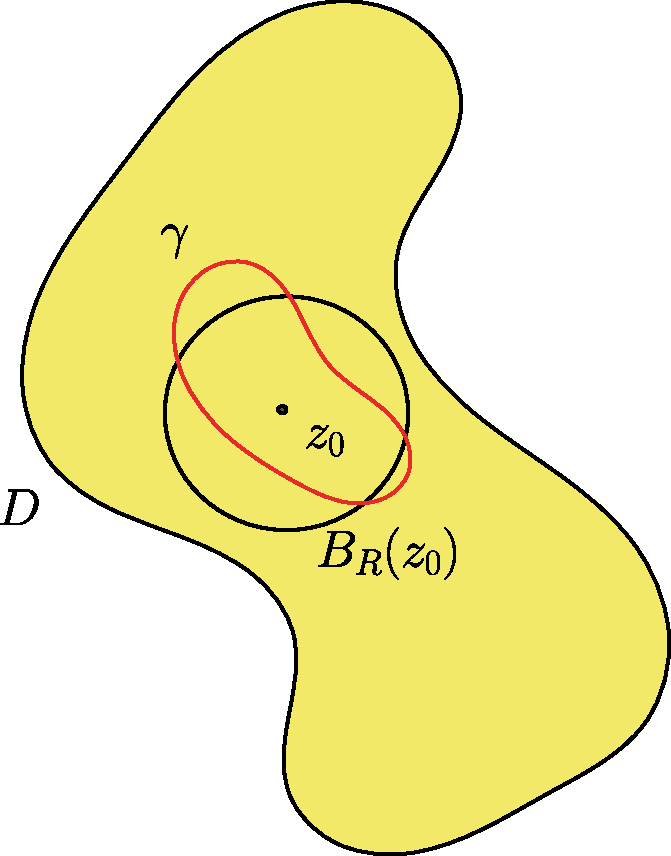
\includegraphics[width=0.3\textwidth]{figure/2026-03-12.pdf}
\caption{representation}
\end{figure}
\begin{parag}{ $ $}
    \begin{subparag}{Intuition}
        The Laurent Series is like a Taylor series but now we include terms with polynomial singularities.

    \end{subparag}
	And as for the Taylor series,  the Laurent series representation is \important{unique}.\\
	$ $\\
	If we find the coefficients $c_n$ by any means (not necessarily by a path integral), then this has to be the Laurent series.
\end{parag}

\begin{definition}
$ $\\
Any Laurent Series splits into a \important{singular} and \important{regular} part
\begin{align*} 
	\sum_{n= -\infty}^{\infty}c_n\left(z - z_0\right)^{n} =  \underbrace{\cdots + \frac{c - 2}{\left(z - z_0\right)^2} + \frac{c - 1}{z - z_0}}_{\text{singular part}} + \underbrace{c_0 + c_1\left(z - z_0\right) + \cdots}_{\text{regular part}}
\end{align*}
In other words, the Taylor series is a Laurent series without singular part.
\end{definition}

\begin{parag}{Example}
    If $f : D \to \mathbb{C}$ holomorphic and $z_0 \in D$ then the Taylor series implies that
	\begin{align*} 
		f\left(z\right) = \sum_{n= 0}^{\infty}x_n\left(z - z_0\right)^{n} =  \sum_{n = 0}^{\infty}\frac{f^{\left(n\right)}\left(z_0\right)}{n!}\left(z - z_0\right)^{n}
	\end{align*}
	The singular part of the Laurent series has to vanish since for all $n \leq -1$ we have 
	\begin{align*} 
		\frac{f\left(\zeta\right)}{\left(\zeta - z_0\right)^{n ! 1}} \text{ is holomorphic near } z_0
	\end{align*}
	By Cauchy's integral formula $\int_{\gamma}\frac{f\left(\zeta\right)}{\left(\zeta - z_0\right)^{n + 1}}d\zetag = 0$\\

\end{parag}
\begin{parag}{Example II}
    For the following function $f : \mathbb{C}\setminus \left\{0\right\} \to \mathbb{C}$ let us find the Laurent series around $z_0 = 0$
	\begin{enumerate}
	    \item $f\left(z\right) =  \frac{1}{z}$ This is already a Laurent series 
			\begin{align*} f\left(z\right) =  \sum_{n =  -\infty}^{\infty}c_nz^{n} \mathspace \mathspace \begin{cases}
			1 \mathspace n = -1\\
			0 \mathspace \text{ otherwise}
			\end{cases}
			 \end{align*}
			 \item $f\left(z\right) = \frac{5z + 1}{z^2} = \frac{1}{z^2} + \frac{5}{z}$ which we can again translate into a Laurent series:
				 \begin{align*} 
					 = \sum_{n = -\infty}^{\infty}c_nz^{n} 
				 \end{align*}
				 Where 
				 \begin{align*} 
					 c_n =  \begin{cases}
					 	1 \mathspace n =  -2\\
						5 =  n = -1\\
						0 \mathspace \text{ otherwise}
					 \end{cases}
				 \end{align*}
	\end{enumerate}
	
\end{parag}







